\subsection{Delay}
Da PM1, PM2 und PM4 �ber eine logische Einheit verbunden sind, welche den TAC startet, muss sichergestellt werden, dass die Signale der drei Photomuliplier Zeitgleich ankommen. Die Zeitversetzung (Delay) der Signale wird �ber die Kabell�nge der Photomuliplier zur logischen Einheit eingestellt.

Es kann angenommen werden, das die Signale von PM3 und PM4 zur selben Zeit ankommen. Deshalb kann das Signal von PM3 gut als Referenz f�r die ersten beiden verwendet werden. F�r die Bestimmung des Delays werden PM1 (bzw. PM2) und PM3 an die logische Einheit angeschlossen, jedoch ohne ein Veto. Die Szintillatoren werden so geschaltet, dass nur bei gleichzeitigem Signal hochgez�hlt wird. Es wird erwartet, das sich ein Plateau ausbildet. Der Delay in der Mitte des Plateaus ist die optimale Einstellung, das sich die Signale an diesem Punkt �berlagern. Damit sich ein m�glichst schmales Plateau ausbildet, m�ssen die Pulse der Diskriminatoren kurz sein. In Abbildung \ref{fig:delay_1} ist zu sehen, dass f�r den ersten Photomulipier kein eindeutiges Plateau identifiziert werden konnte. Deshalb musste das Delay mit dem Oszilloskop eingestellt werden, um sicherzustellen, dass sich die beiden Signale �berlappen. F�r den ersten Photomuliplier wurde mit dem Oszilloskop ein Delay von 9ns bestimmt. In Abbildung \ref{fig:delay_2} sind die Messdaten f�r den zweiten Photomuliplier zu sehen. Im Bereich von 20 bis 28ns ist ein Plateau zu erkennen, das Delay wurde mit dem Wert (24ns) in der Mitte des Plateaus angenommen. Das Delay von 24ns f�r den zweiten Photomuliplier wurde zus�tzlich mit dem Oszilloskop bestimmt und konnte best�tigt werden.

\begin{figure}[H]
	\centering
  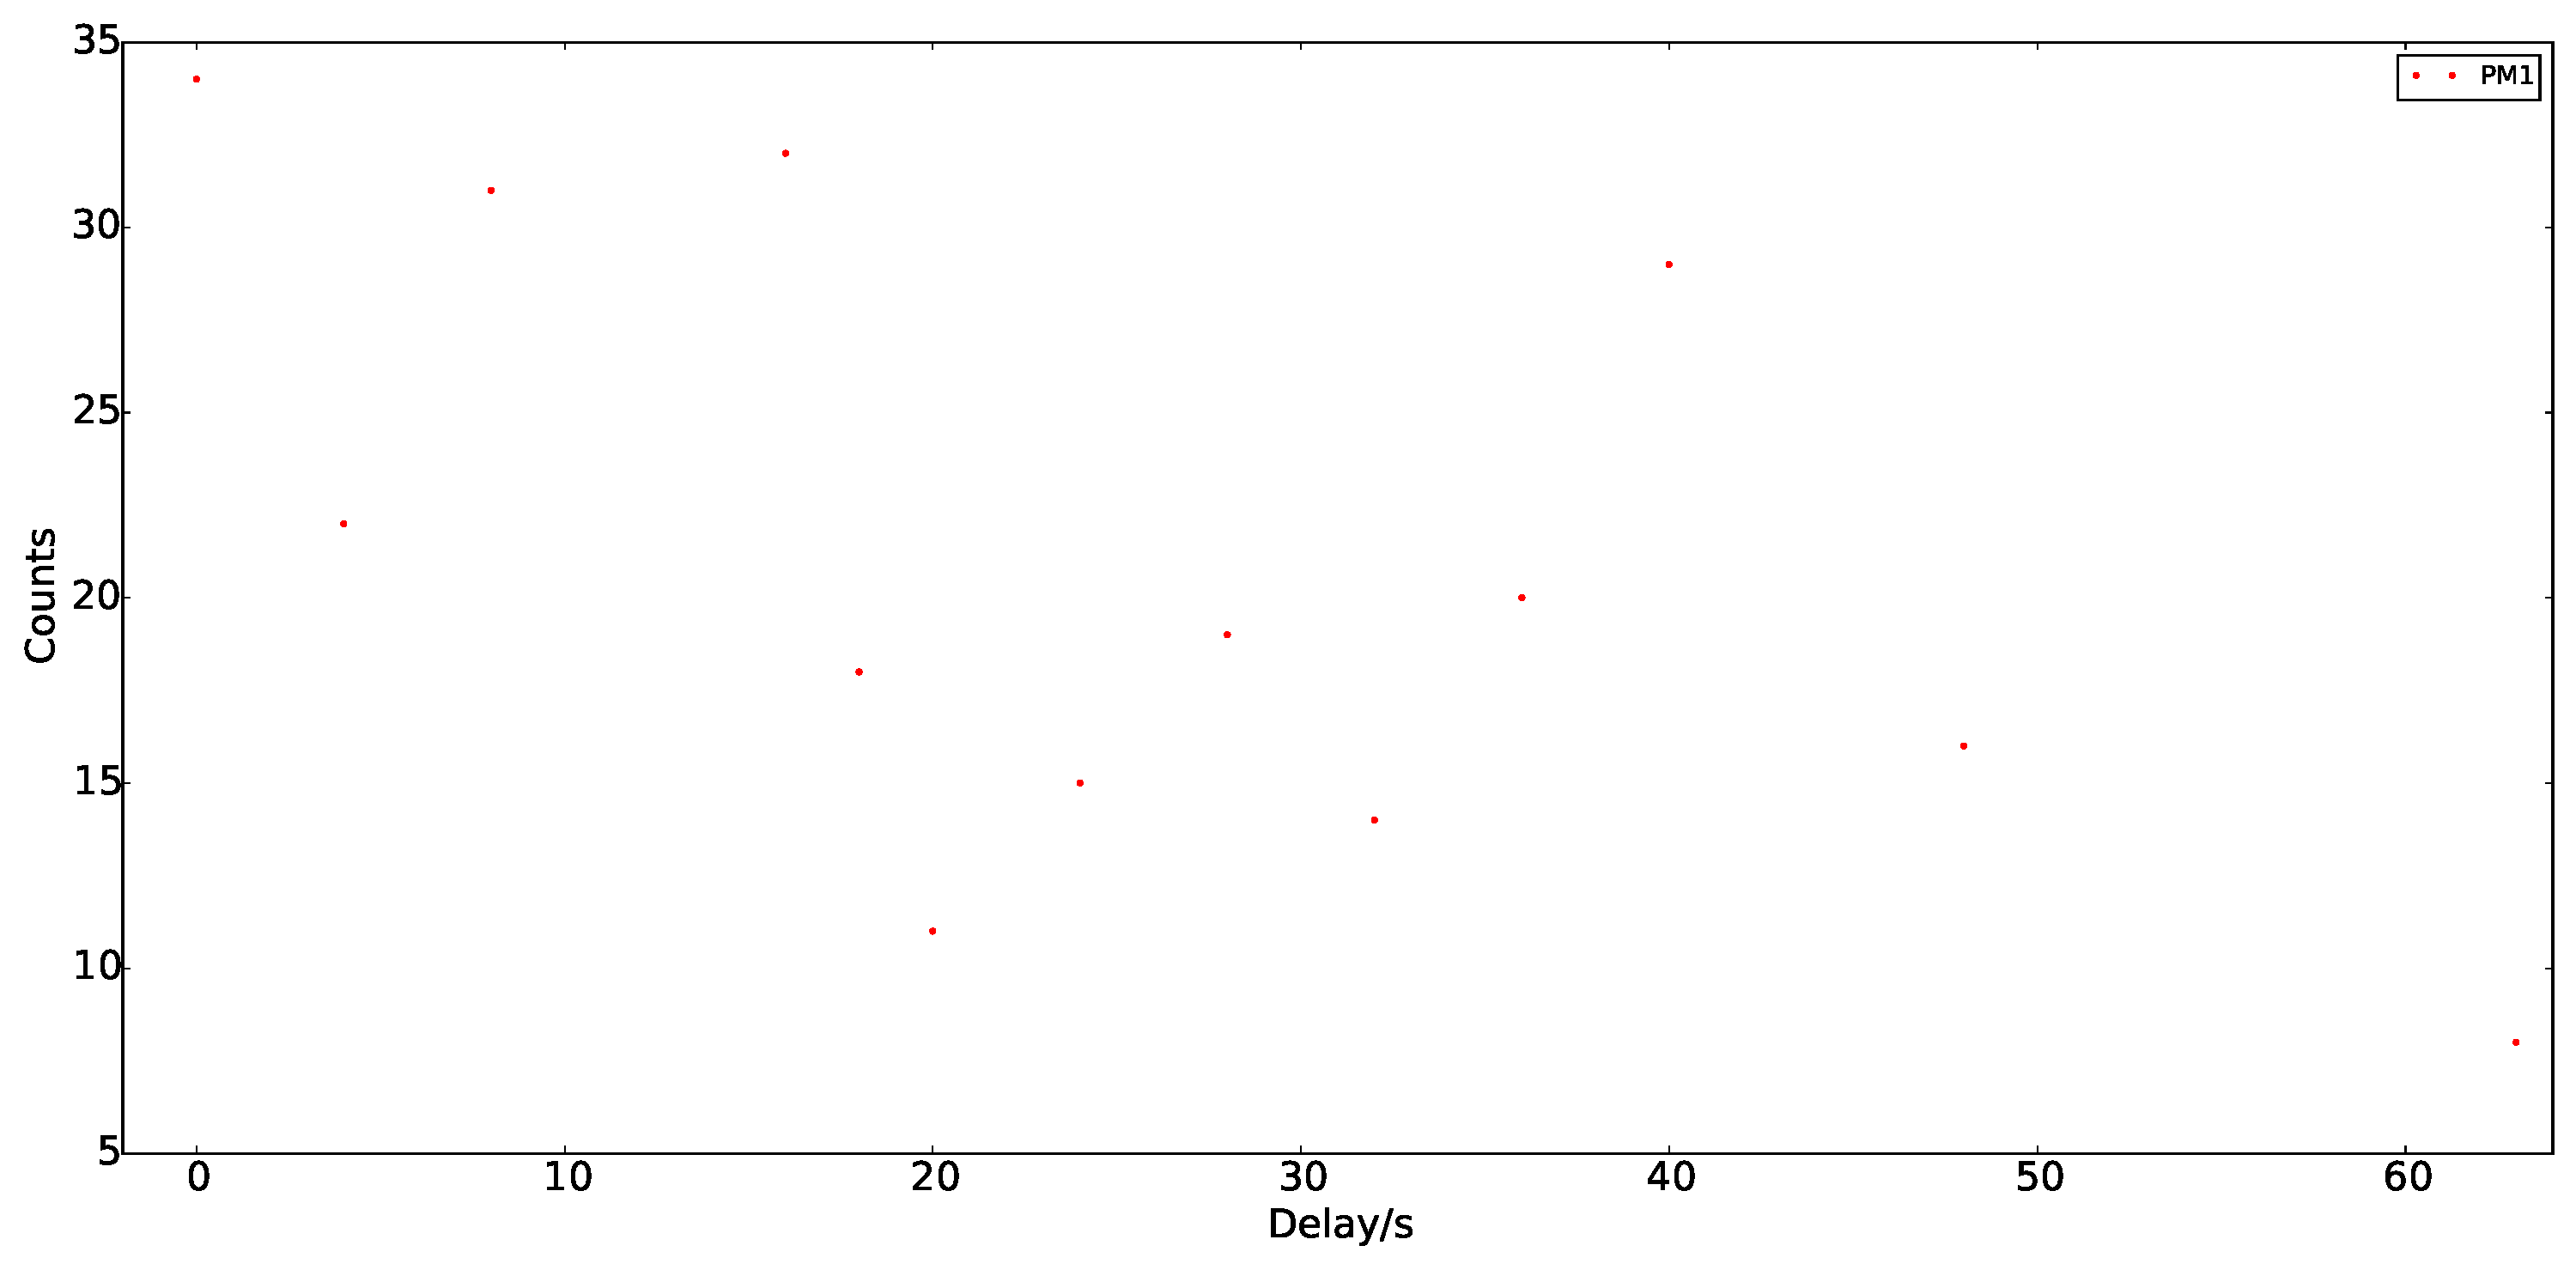
\includegraphics[scale=0.33]{delay_1.pdf}
	\caption{Counts in Abh�ngigkeit vom Delay f�r die ersten Photomuliplier, es ist kein eindeutiges Plateau zu erkennen. Deshalb wurde das Signal mit einem Oszilloskop betrachtet und ein Delay von 9ns bestimmt.}
	\label{fig:delay_1}
\end{figure}


\begin{figure}[H]
	\centering
  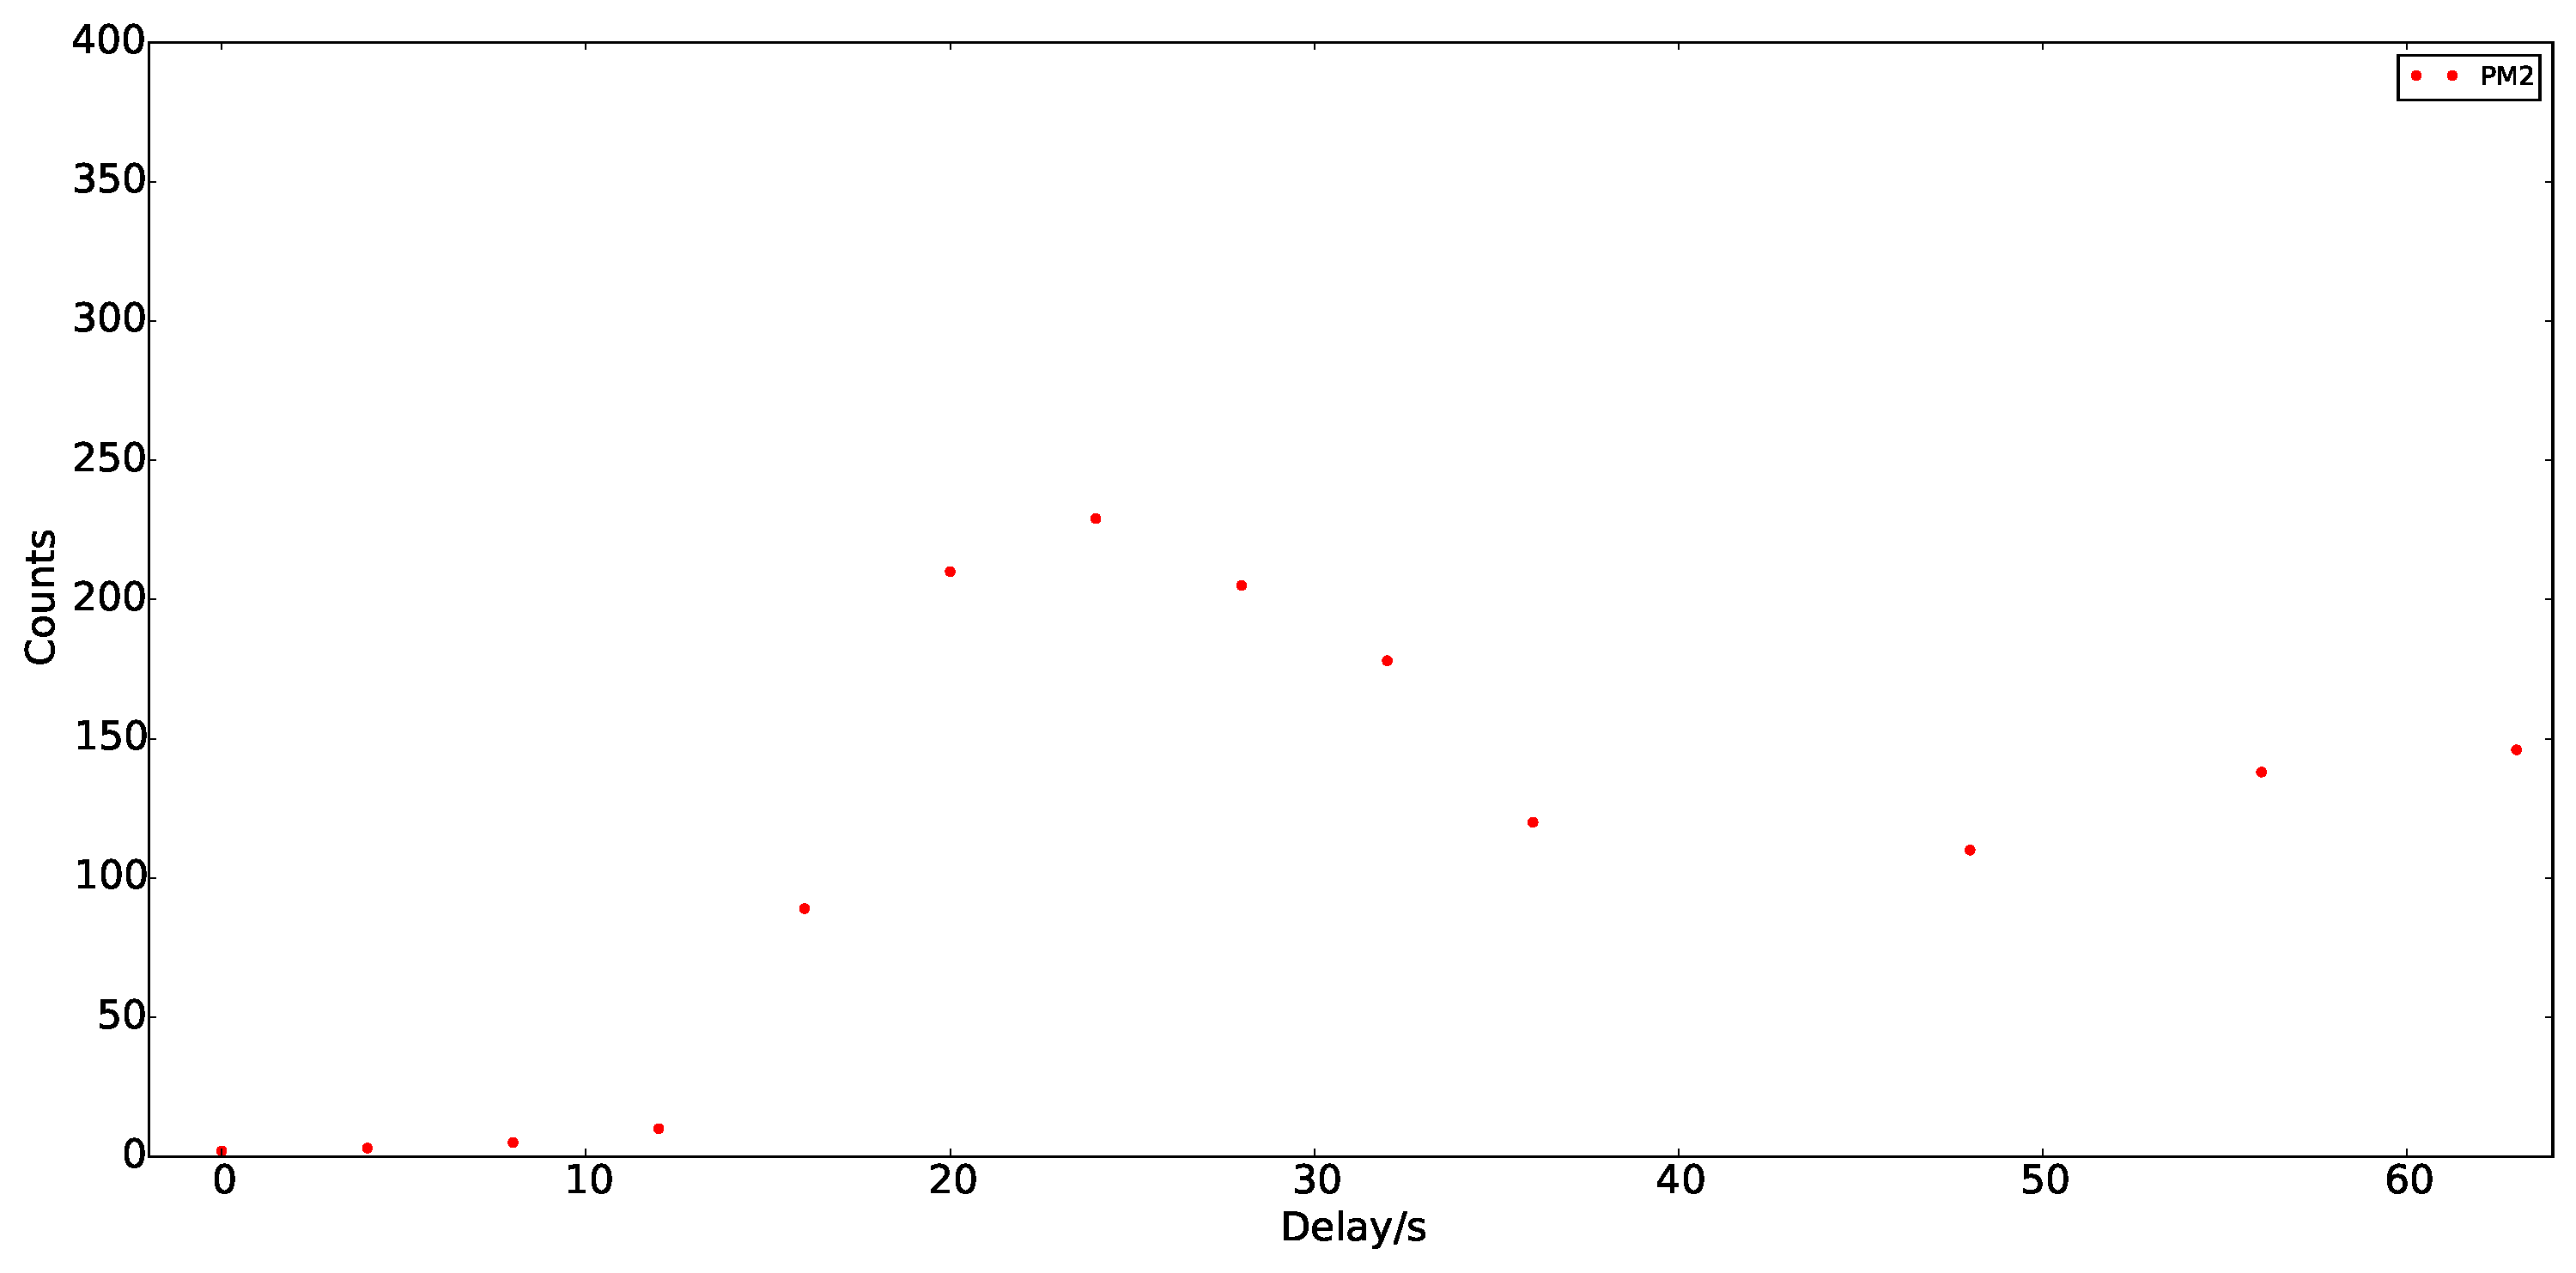
\includegraphics[scale=0.33]{delay_2.pdf}
		\caption{Counts in Abh�ngigkeit vom Delay f�r die ersten Photomuliplier. Ein Plateau ist im Bereich von 20 bis 28 ns zu erkennen. Das Delay wurde mit 24 ns, in der Mitte des Plateaus bestimmt. dieser Wert wurde mit dem Oszilloskop verifiziert.}
	\label{fig:delay_2}
\end{figure}

Es ergeben sich die Delays in Tabelle \ref{tab:delay}.

\begin{table}[H]
	\centering
	\caption{Optimal bestimmtes Delay f�r PM1 und PM2}
	\label{tab:delay}
	\begin{tabular}{|c|c|}
	\hline Photomuliplier & Delay [ns] \\ \hline
	\hline PM1 & 9 \\ 
	\hline PM2 & 24 \\ 
	\hline 
	\end{tabular} 
\end{table}

Das Oszilloskopbild Abb. \ref{PMT2Delay} zeigt, dass die Signale beim zweiten Photomultiplier �bereinander liegen. Auff�llig war, dass trotz Abschlusswiderstand verschobene Signale angezeigt wurden, die eigentlich nicht zu sehen sein sollten.
\begin{figure}[H]
\centering
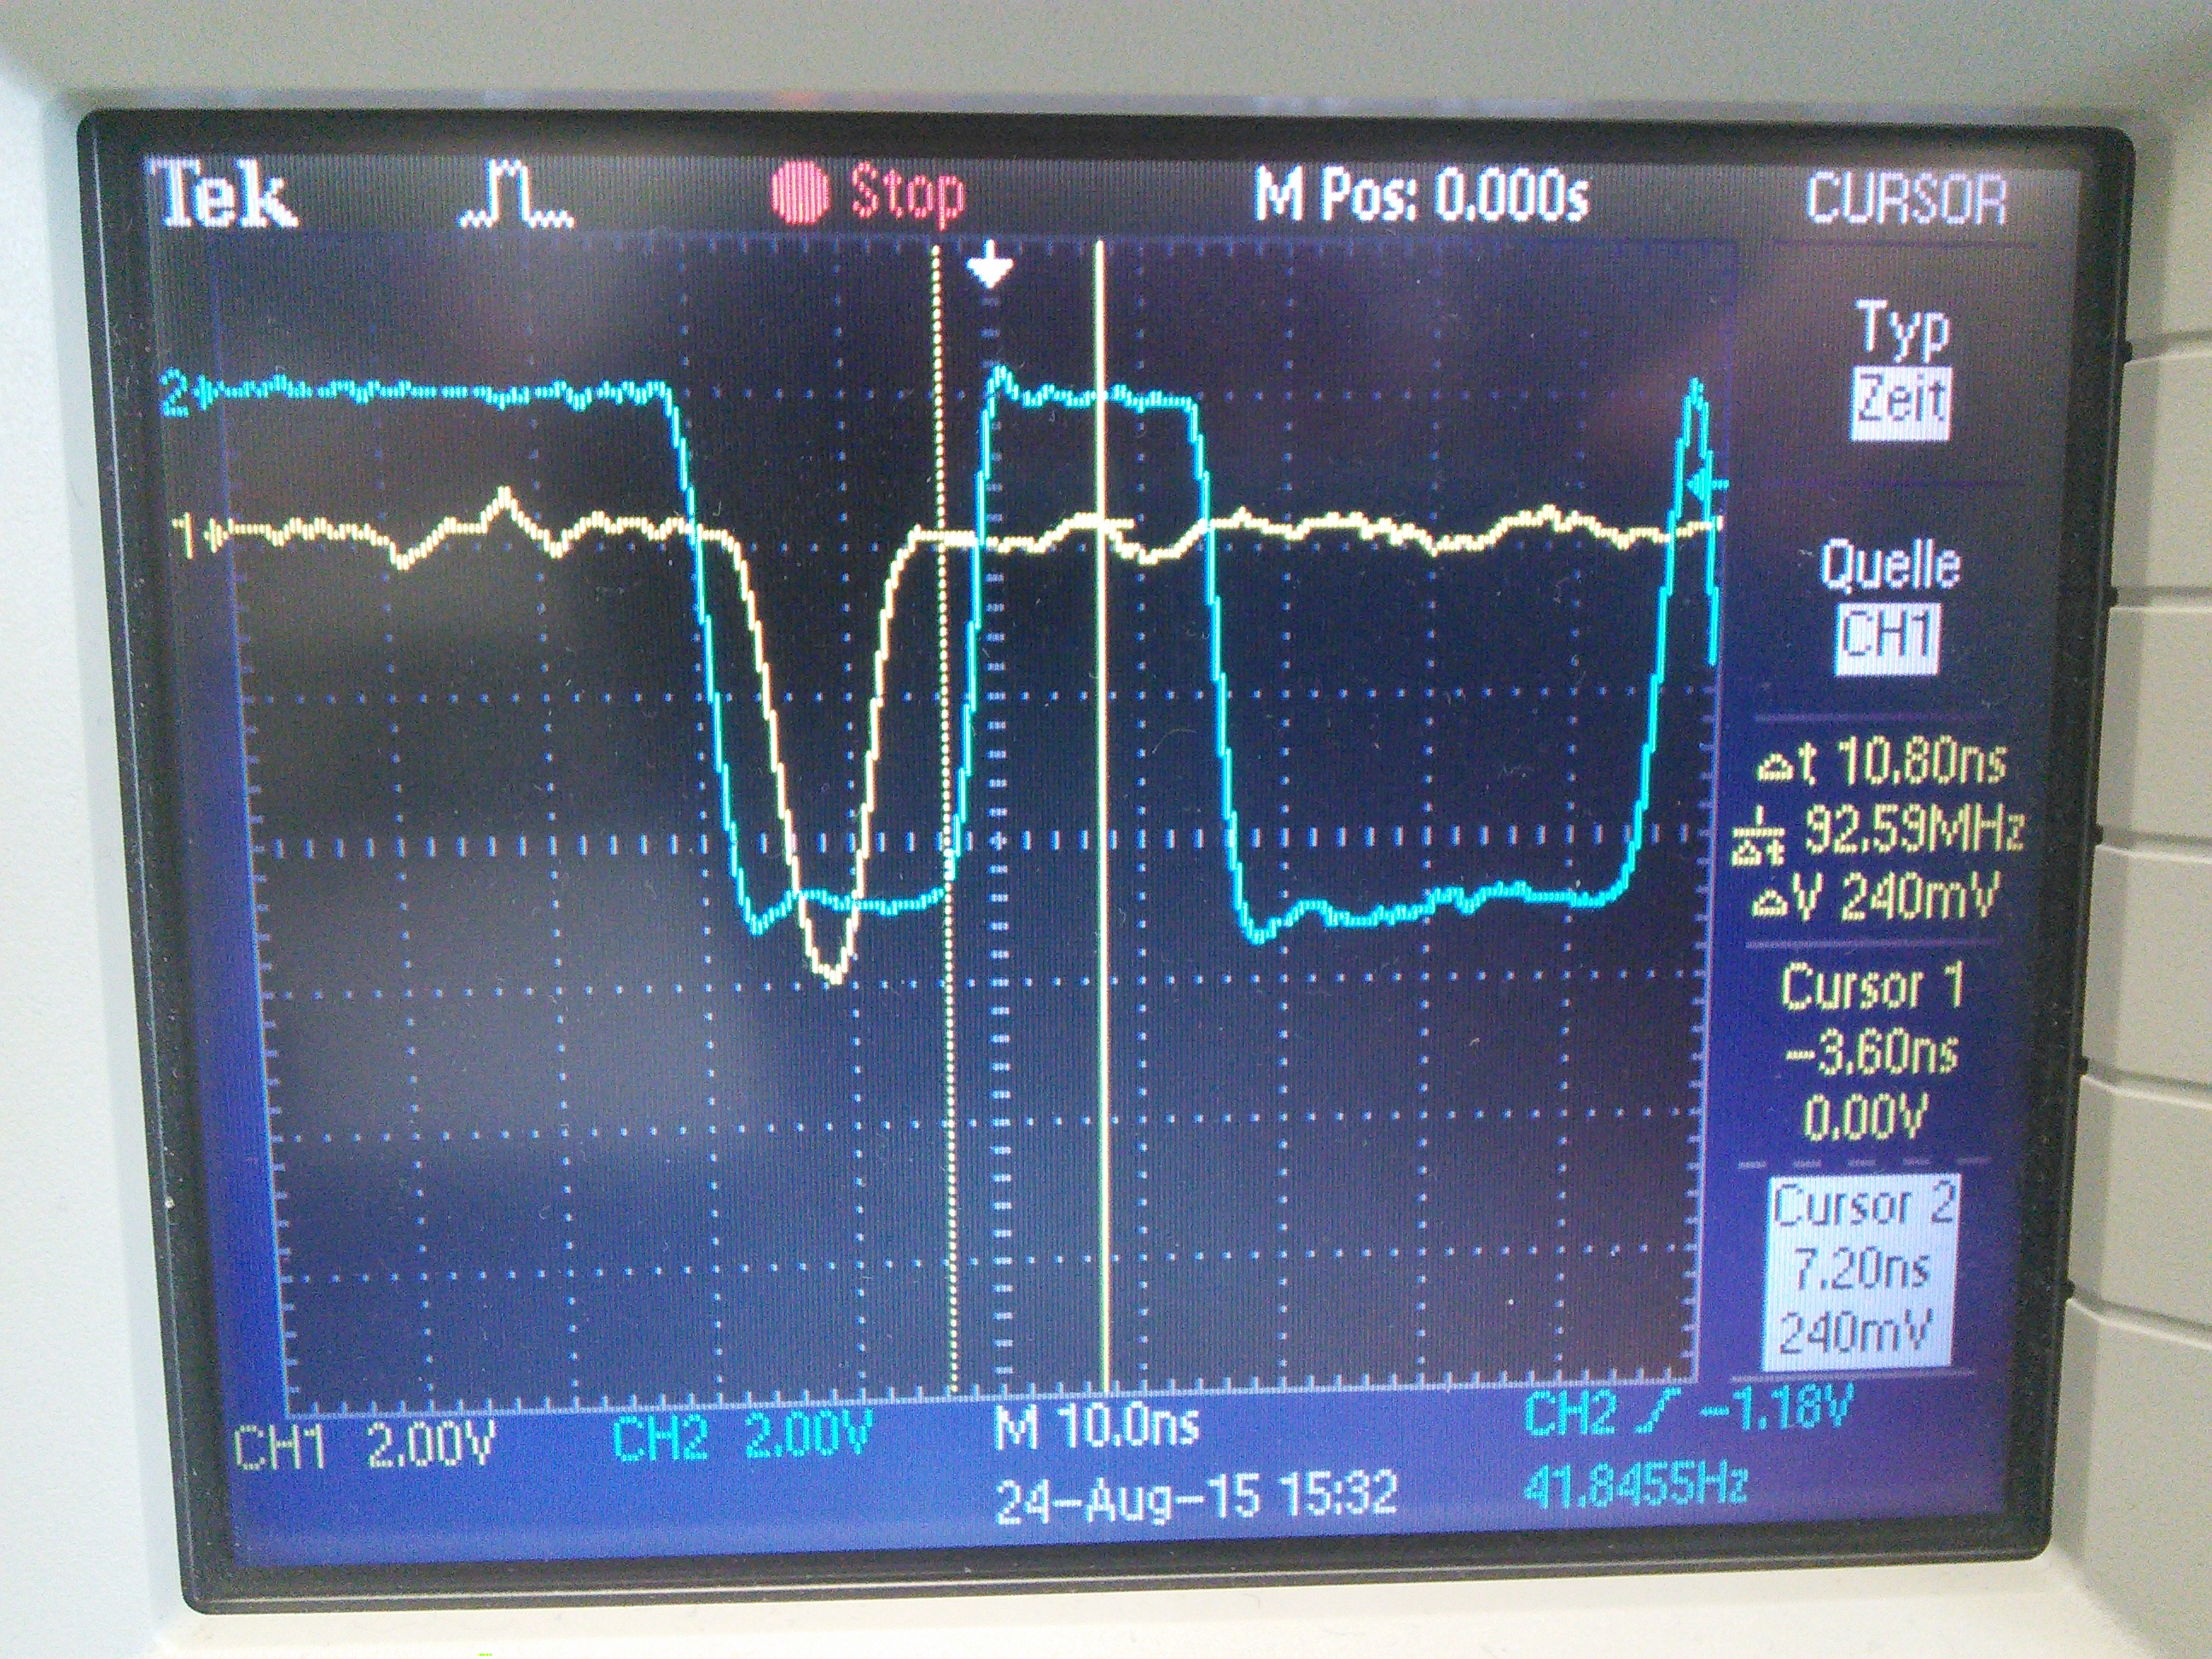
\includegraphics[scale=0.12]{DelayPMT2}
\caption{Oszilloskopbild Delay PMT 2}
\label{PMT2Delay}
\end{figure}